%\lstinputlisting{satellite.py}
\section{Satellite galaxies around a massive central}
The exercise is done in the script satellite.py. The necessary explanations of the methods used are in the comments of the code. For the purpose of this task, we implement a Random Number Generator (RNG) as follows: \lstinputlisting[firstline=10,lastline=59]{satellite.py}
For question (a), we do the following: \lstinputlisting[firstline=62,lastline=135]{satellite.py} The normalization factor A we obtain is the following: \lstinputlisting{normalization.txt}.
For question (b), we generate 3D satellite positions that statistically follow the satellite profile $n(x)$. We sample them from the probability density function $p(x)$, using the inverse transform sampling. We compare the distribution of the sampled points with $N(x)$, the analytical function describing the number of galaxies in a shell of thickness $dx$ at a given distance $x$. From Fig.\ref{fig:n_vs_hist}, we can see that the sampled points match the expected distribution. Nevertheless, we can see how the samples are not present in the first interval of $x$ values. Inverse sampling works by transforming uniform random numbers into samples from the desired distribution, using the cumulative distribution function (CDF) of the PDF. The CDF maps values from the sample space to the interval [0, 1], and its inverse can be used to map values from [0, 1] back to the sample space. In the case of smaller values, a small range of uniform random numbers can map to a large range of small values in the sample space, leading to undersampling in these regions. This might explain why there is a discrepancy at smaller values in our histogram.

\begin{figure}[h!]
  \centering
  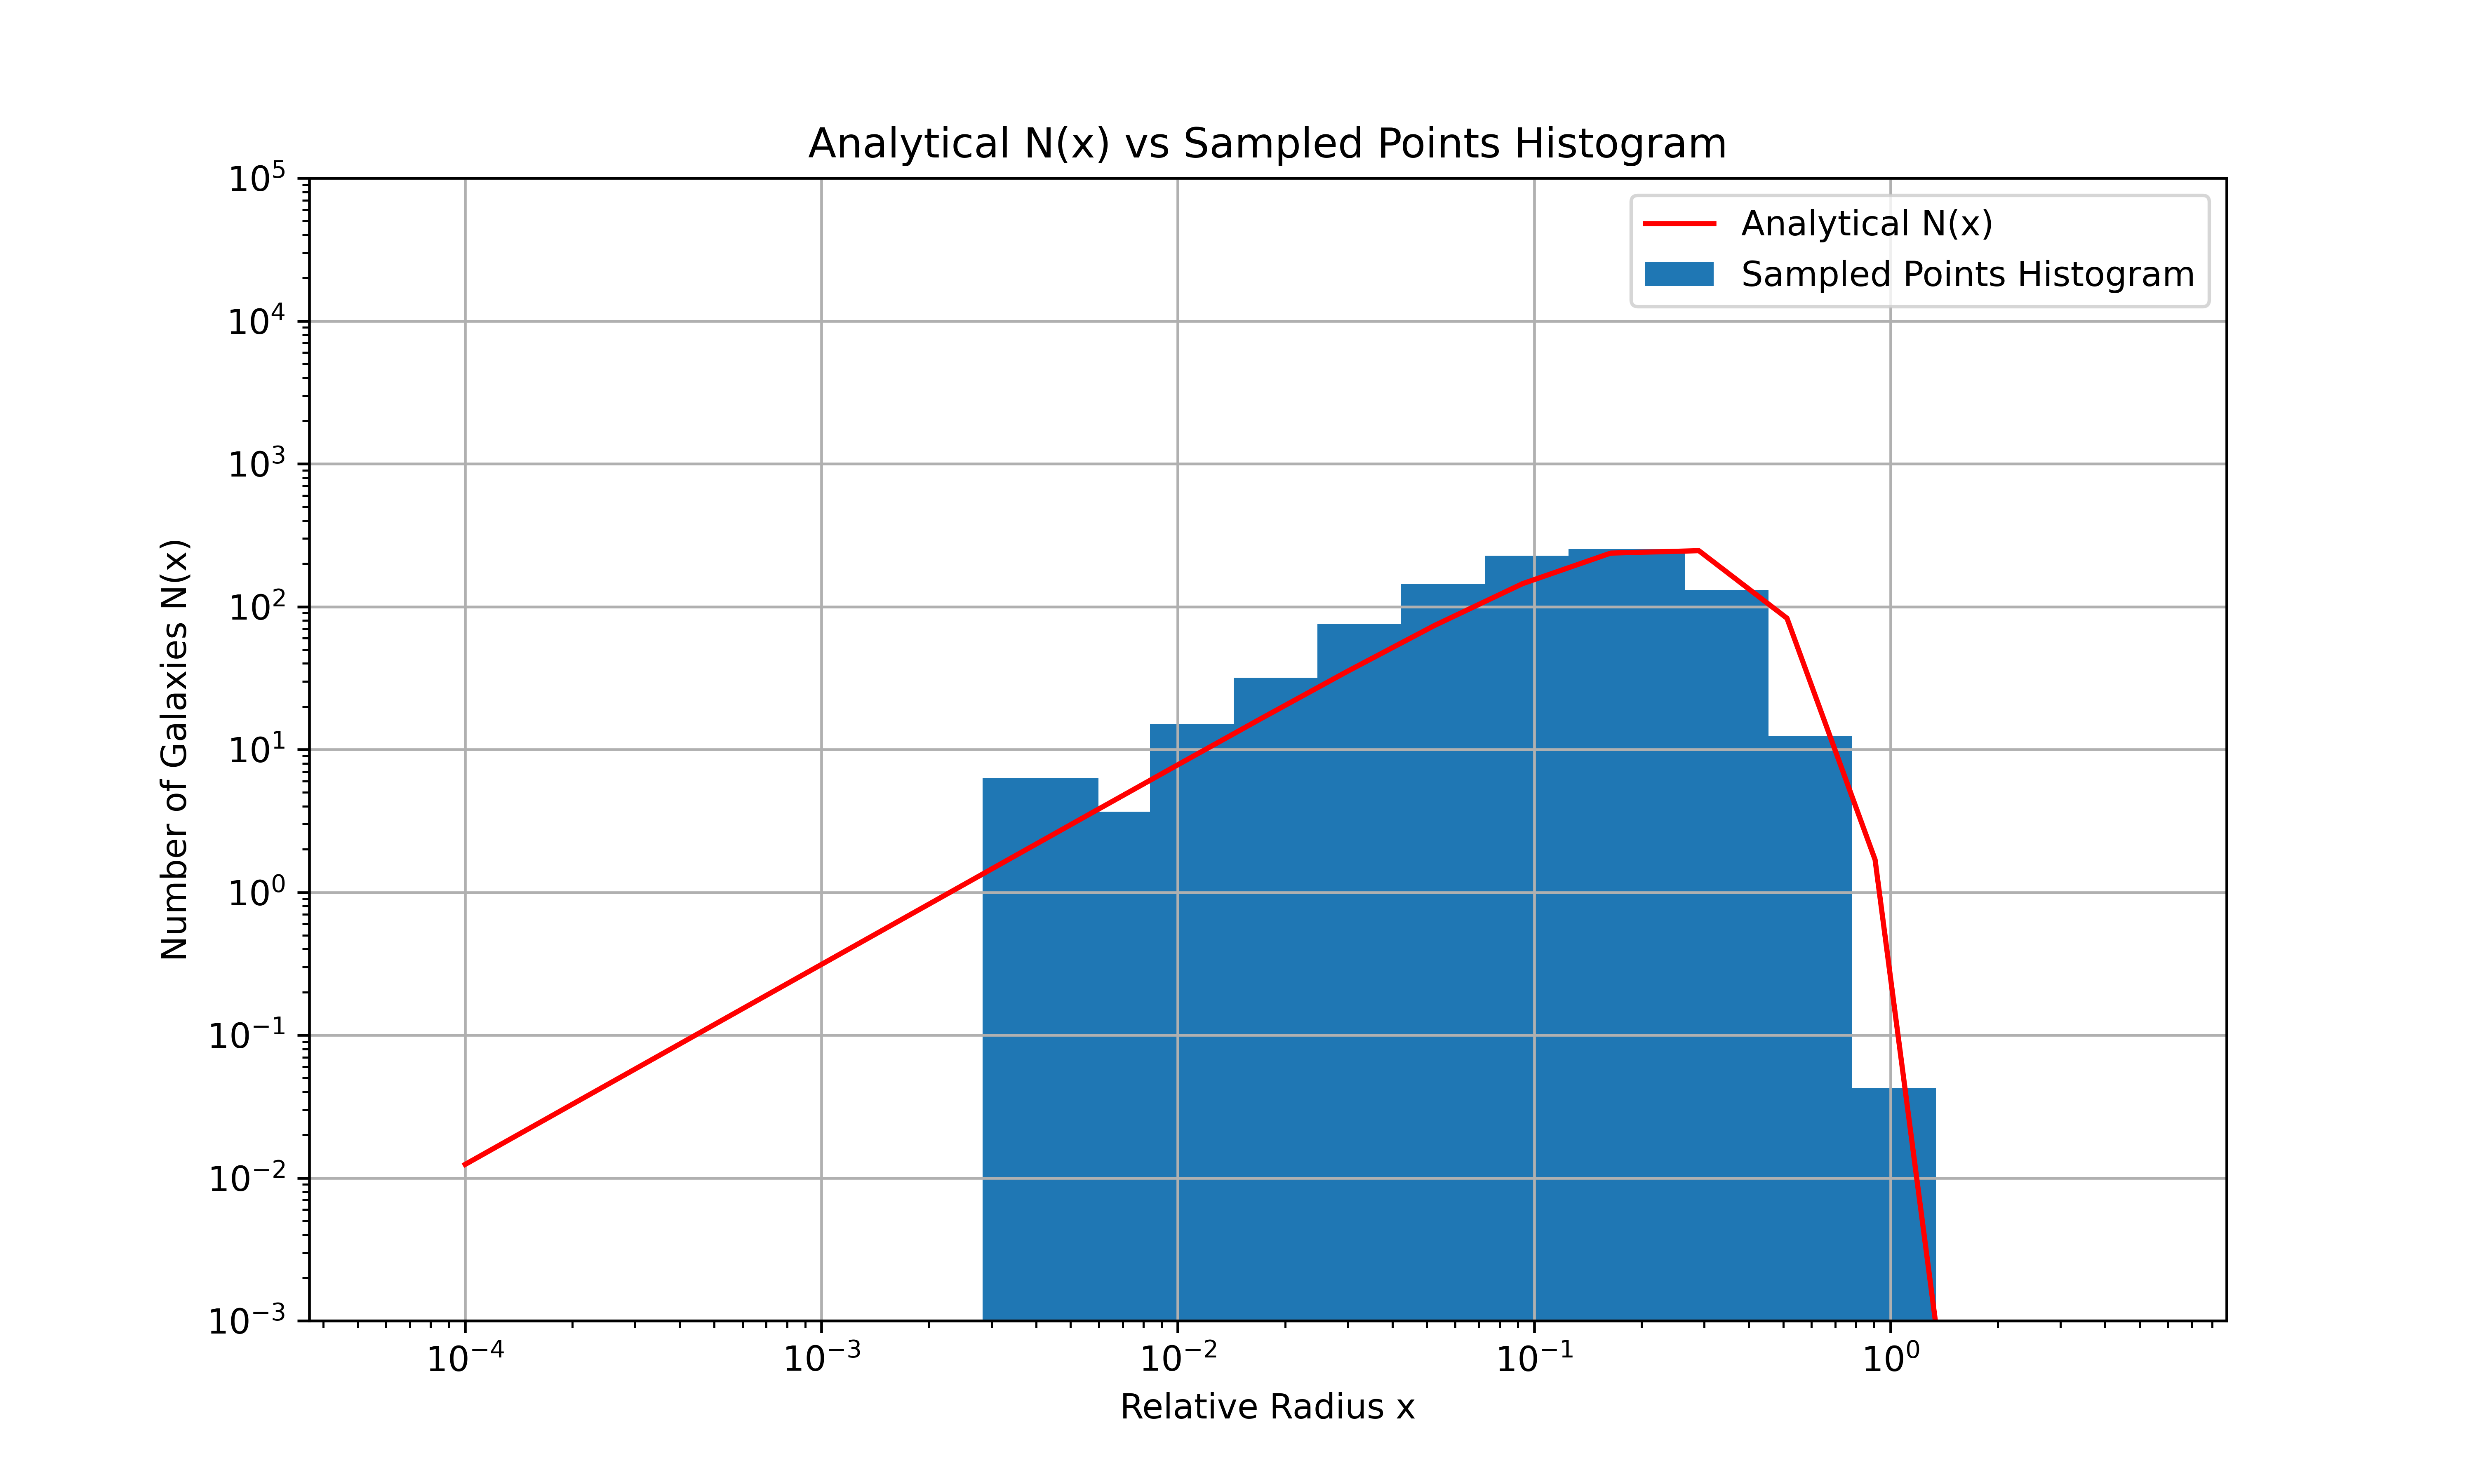
\includegraphics[width=0.9\linewidth]{./plots/my_solution_1b.png}
  \caption{Plot in logarithmic scale showing $N(x)$, function of the number of galaxies at given distance $x$, and the histogram of the 10000 sampled points. The sampled points match the analytical distribution, but there is a problem of undersampling in the region of smaller radii.}
  \label{fig:n_vs_hist}
\end{figure}

For question (c), we select 100 random galaxies from the ones sampled in point (b), using Reservoir method. It is a sampling algorithm that chooses a random sample, without replacement, of $k$ items from a population of unknown size $n$ in a single pass over the items. The 100 drawn galaxies are ordered from smallest to largest radius. The number of galaxies within a radius $x$ are shown in Fig. \ref{fig:cum_galaxies}. The radii selected are starting from higher values because of the previous undersampling. The increasing trend makes sense as the number of galaxies within a given radius should increase as the radius increases.

\begin{figure}[h!]
  \centering
  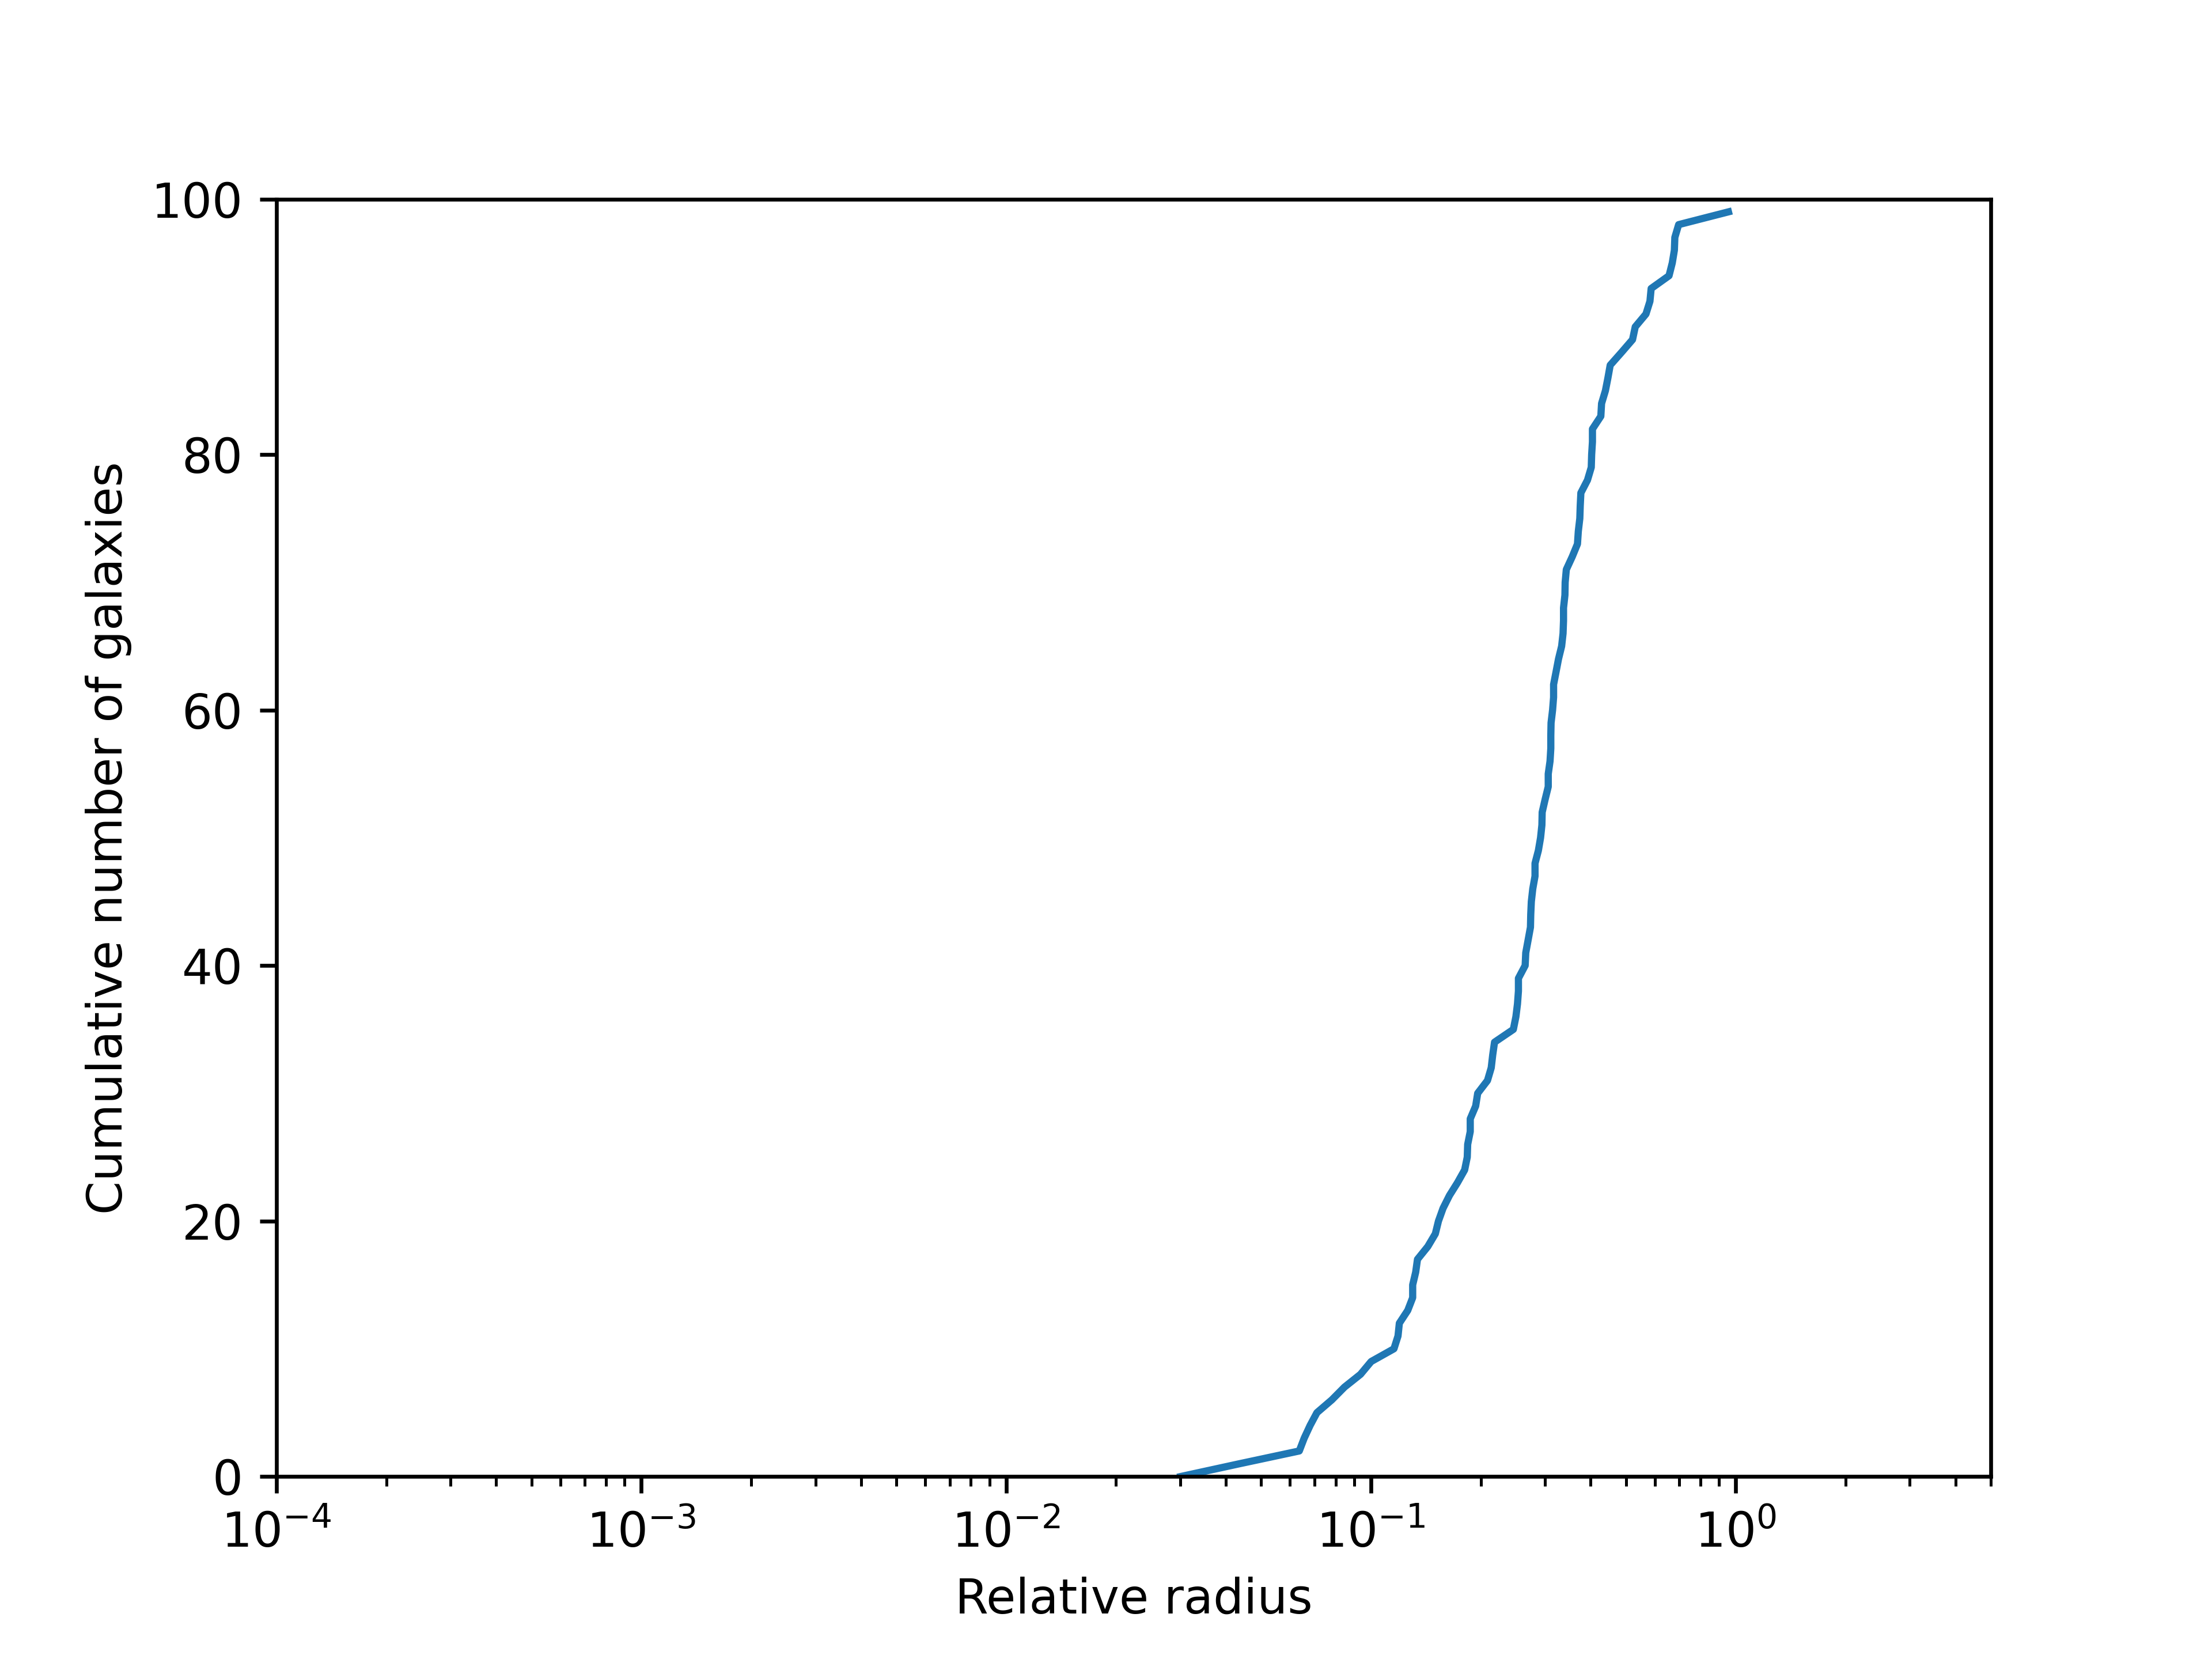
\includegraphics[width=0.9\linewidth]{./plots/my_solution_1c.png}
  \caption{Plot showing the cumulative number of galaxies randomly selected with respect to the relative radius $x$. The number of galaxies progressively increases with larger distances.}
  \label{fig:cum_galaxies}
\end{figure}

For question (d), we compute the derivative of the function $n(x)$ using both the Ridders' method and the analytical procedure. The obtained results can be seen in: \lstinputlisting{derivative.txt}


\section{Heating and cooling in HII regions}

